\section{Performance estimation}\label{capitolo4}
Per verificare se un sistema rispetta o no le specifiche è necessario testare il sistema una volta realizzato. Esistono diversi meccanismi per effettuare questi test ma possiamo dividerli in due categorie, i metodi \emph{host profile} nei quali la strumentazione è eseguita su una macchina diversa da quella testata detta appunto \emph{host} e  metodi \emph{target profile} nei quali le informazioni vengono prelevate direttamente sulla piattaforma o so un prototipo. Le analisi di tipo \emph{target profile} sono utilizzate per misurare le performance di un sistema soprattutto quando alcune parti dell'applicazione sono realizzate tramite librerie proprietarie delle quali non se ne conosce l'efficienza, oppure nel caso in cui i valori di ingresso sono disponibili solo per la macchina target ma soprattutto nel caso in cui le tecniche di ottimizzazione richiedano un'analisi più accurata. In alcuni casi è anche possibile fare delle misurazioni anche su architetture incomplete, quando ad esempio l'architettura finale non è ancora disponibile oppure quando si vogliono testare più soluzioni per alcune parti del sistema.\\
Per effettuare le misurazioni sulla macchina target si sfruttano le librerie \emph{openMP}, in una prima fase il progettista inserisce i costrutti \emph{pragmas} nelle sezioni di codice che richiedono di essere misurati, successivamente questi costrutti vengono sostituiti da opportune istruzioni per la misurazione, nella fase di \emph{compilazione ed esecuzione} il codice viene compilato ed eseguito sull'architettura designata. Nella terza fase si collezionano tutti i dati e si confrontano con quelli già raccolti per stimare le performance dell'architettura finale. Un esempio di questo flusso è mostrato in \figurename\,\ref{fig:metodoflow}.\\
\begin{figure}
\centering
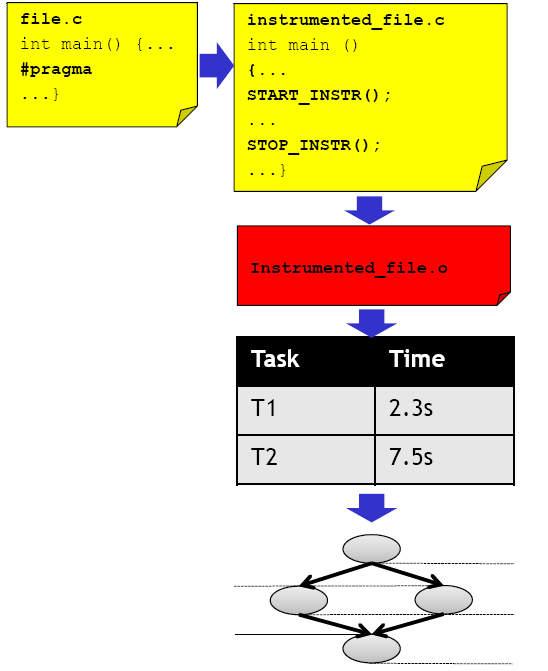
\includegraphics[scale=0.4]{img/metodoflow.png}
\caption{Flusso di raccolta dei dati}\label{fig:metodoflow}
\end{figure}
L'aggiunta delle istruzioni \emph{pragma} non influenza l'indipendenza del codice dall'architettura, è possibile tuttavia personalizzare il codice per una singola architettura tramite la definizione di un file di configurazione.\\
In alcuni casi l'analisi sull'architettura target non è fattibile, o perchè l'architettura non è ancora disponibile o perchè il progettista deve scegliere tra una vasta serie di elementi diversi. Sono state introdotte perciò delle metodologie per la creazione automatica di modelli per l'analisi delle performance i quali non richiedono alcuna conoscenza sull'architettura targhe, sfruttano il \emph{GCC Register Transfert Language} ma soprattutto permettono l'\emph{host profiling}. In \figurename\,\ref{fig:gccschema} vediamo come il compilatore esegue la trasformazione del codice sorgente in codice assembly.
\begin{figure}
\centering
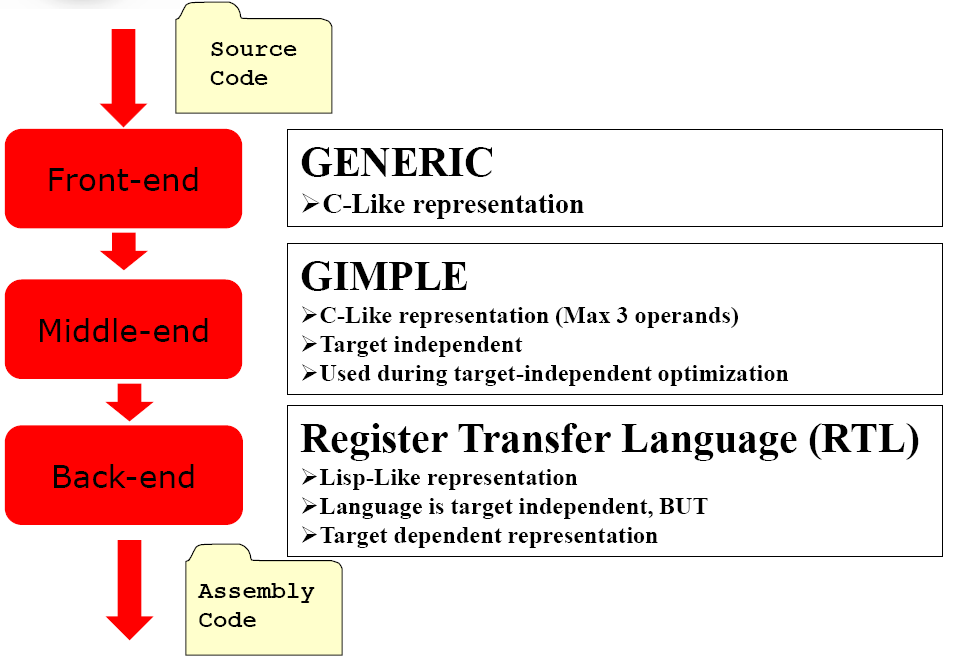
\includegraphics[scale=0.4]{img/gccschema.png}
\caption{Flusso di compilazione in GCC}\label{fig:gccschema}
\end{figure}
Il modello lineare è un'approssimazione del modello reale che non tiene in considerazione alcuni aspetti architetturali come il VLIW o la cache. I vantaggi di questo modello sono il fatto che esso è adattativo, semplice e leggibile e abbastanza accurato per essere usato per alcune fasi della progettazione.
Dati i modelli esistono diversi tipi di analisi che possono essere eseguite:
\begin{itemize}
\item \emph{Dinamica} che permette di tenere in considerazione come le performance dipendano dai dati 
\item \emph{RTL} che permette di considerare alcuni aspetti architetturali della macchina targhet
\item \emph{Sequenziale} permette di tenere in considerazione aspetti architetturali specifici come la pipeline, tuttavia questo tipo di analisi è estremamente difficile in quanto è difficile modellare gli effetti di tali aspetti.
\end{itemize}
Un simulatore o una piattaforma reale non è disponibile durante le fasi iniziali della progettazione dobbiamo costruire cosi un modello matematico per ogni singolo elemento. Tale procedimento richiede che il compilatore estragga dei dati per ogni elemento, tuttavia in alcuni casi alcuni processori utilizzano un loro compilatore proprietario che non permette di di estrarre rappresentazioni intermedie. Una soluzione allora è quella di approssimare la soluzione del compilatore proprietario a quella di GCC per fare ciò si utilizza una rappresentazione intermedia denominata \emph{GIMPLE} la quale è indipendente dall'architettura. Tuttavia il compilatore proprietario e GCC effettuano ottimizzazioni differenti.
\subsection{Task graph performance estimation}
Combinando i risultati delle precedenti analisi sui singoli task si cerca di stimare le performance globali, tuttavia l'esecuzione di alcuni task è correlata ad altri come nell'esempio di \figurename\,\ref{fig:taskgraph}
\begin{figure}
\centering
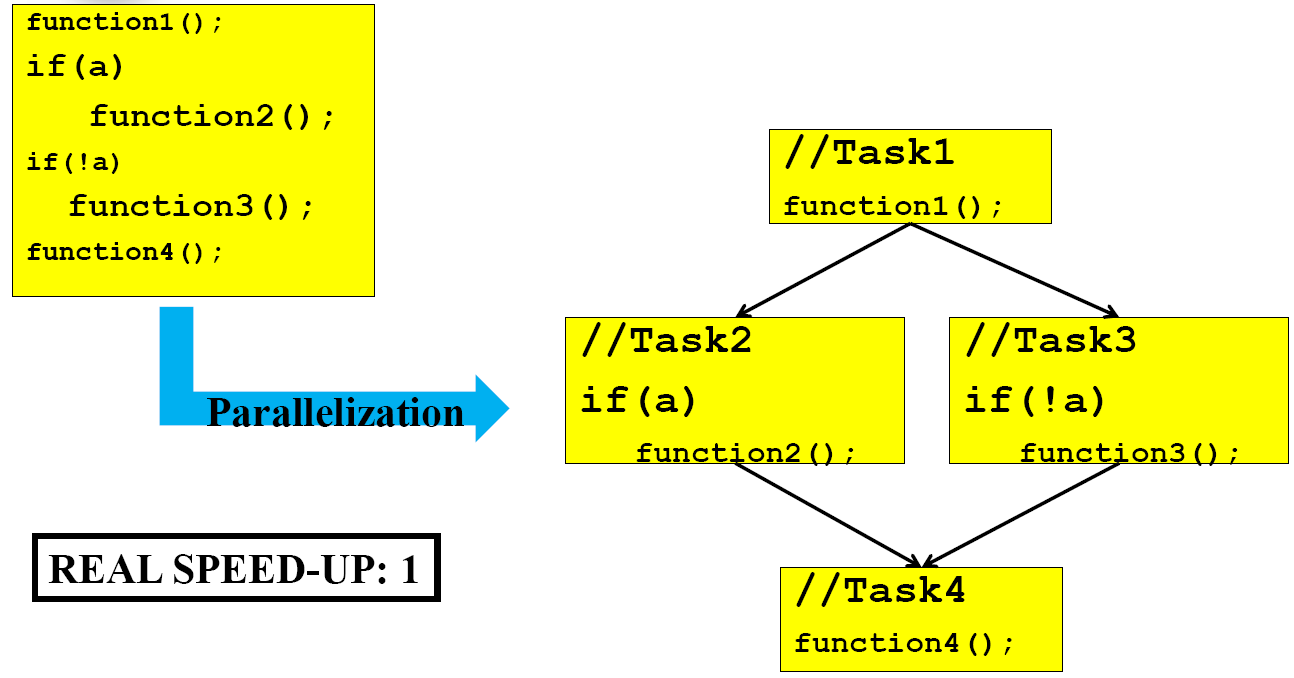
\includegraphics[scale=0.3]{img/taskgraph.png}
\caption{Esempio di grafico dei task}\label{fig:taskgraph}
\end{figure}
In questo metodo si tiene conto sia del percorso di esecuzione sia della topologia del task graph, il valore globale è dato dalle performance stimate moltiplicate per il loro peso sommate al contributo fornito da ogni percorso di esecuzione. Il contributo di ogni percorso è calcolato considerando le performace sul task graph quando solo il percorso di esecuzione è attivo. Il costo di creazione e distruzione dei task è costante. La frequenza dei diversi percorsi è ottenuta tramite profilazione dell'appllicazione tramite simulazione, ogni percorso è identificato da un intero, i percorsi possibili quelli che cominciano nel punto d'entrata e finiscono all'uscita della fnzione. Un esempio di tale meccanismo è mostrato in \figurename\,\ref{fig:taskestiamtion1} e \ref{fig:taskestiamtion2} dalla quale possiamo ricavare che:
$$\dfrac{(E_{p1}*F_{1})+(E_{p2}*F_{2})}{F_1+F_2}=\dfrac{(3000*0.2)+(3000*0.8)}{0.2+0.8}=3000$$
\begin{figure}
\centering
\subfigure[]{
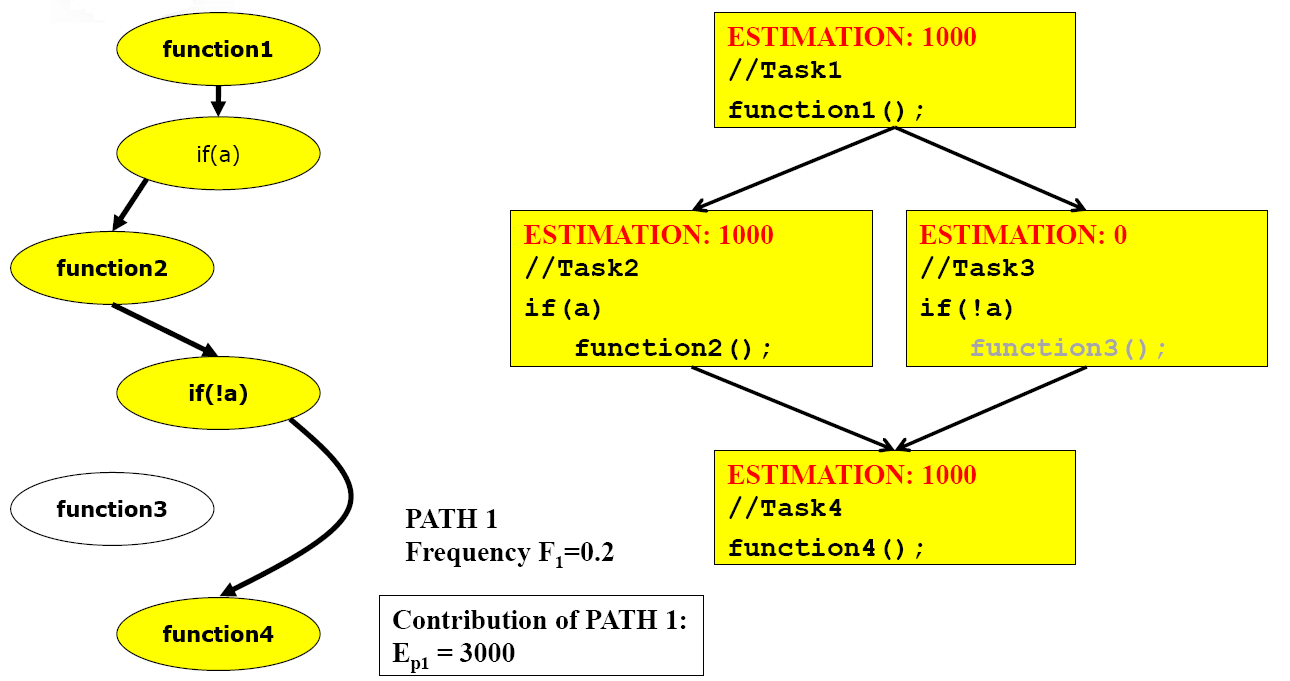
\includegraphics[scale=0.4]{img/taskestimation1.png}
\label{fig:taskestiamtion1}
}
\subfigure[]{
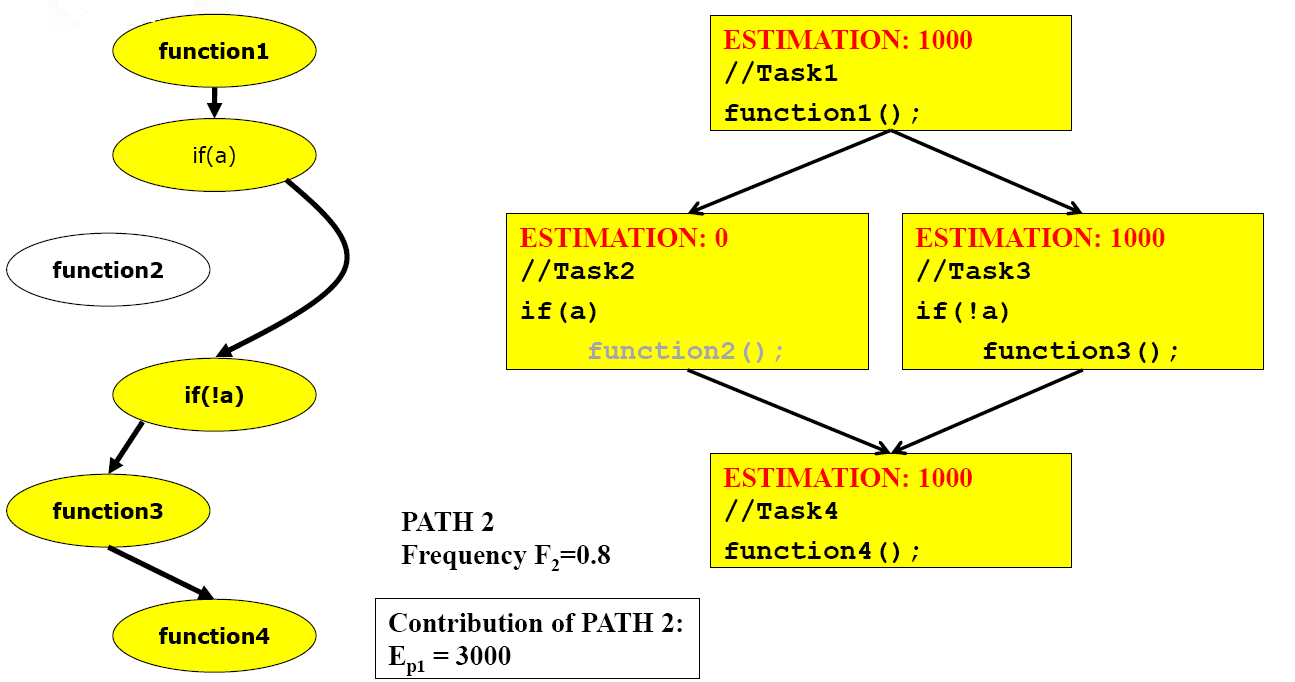
\includegraphics[scale=0.4]{img/taskestimation2.png}
\label{fig:taskestiamtion2}
}
\caption{Attivazione dei percorsi}
\end{figure}